\documentclass[a4paper,10pt]{article}
\usepackage[utf8]{inputenc}
\usepackage{fullpage}
\usepackage{cite}
\usepackage{graphicx}
\usepackage{wrapfig}
\usepackage{url}
\DeclareGraphicsExtensions{.pdf,.eps,.svg,.pgm, .png}
    % EXTREMELY COMMON LaTeX PACKAGES TO INCLUDE:
    \usepackage{amsmath,amsthm, amsfonts,amssymb} % For AMS Beautification
    \usepackage{setspace} % For Single & Double Spacing Commands
    \usepackage[linktocpage,bookmarksopen,bookmarksnumbered,% For PDF navigation
		pdftitle={Group 2: Sotiriou et. al.},%   and URL hyperlinks
		pdfauthor={Department of Electronic and Computing Systems},%
		pdfsubject={UC },%
		pdfkeywords={UC}]{hyperref}
           \usepackage{caption3} % load caption package kernel first
    \DeclareCaptionOption{parskip}[]{} % disable "parskip" caption option
    \usepackage[small]{caption}
\usepackage{amsmath}
\usepackage{amsfonts}
\usepackage{amsthm}
\usepackage{float}
\usepackage[section]{placeins}
%opening
\title{Assessing Histological Grades of Primary Breast Cancer Using Gene Signatures}
\author{Priyanka Arora, Lee Carraher,Ben Landis, Li Jing, Samuel Schmidt}
\begin{document}

\maketitle

\begin{abstract}
This paper is a re-Analysis of the Sotiriou et. al. paper on using tumor 
histological grade expressed gene signatures for breast cancer 
prognosis\cite{Sotiriou}. The principle assumptions of this process are that
the classification of histological grade and tumor progression has a strong 
correlation with the length of survival time. Furthermore, we suggest grade 2
tumors are misclassified grade 1 or grade 3 tumors. The result of developing 
better gene signatures for classifying tumor grades can further
assist in diagnosis and treatment options for breast cancer patients.


\end{abstract}


\section{Background}   
Breast Cancer is the most common malignancy among women and is the second 
leading cause of cancer death.The American Cancer Society estimated 234,580 new 
cases of breast cancer in US, 2013 and 40,030 deaths related to breast cancer. 
The incident rate of new cases of breast cancer is highest 
for Whites and second highest for African Americans \cite{henderson1}.  Breast cancer incidence is lowest for those of American Indian/Alaska Native, 
Asian American/Pacific Islander, and Hispanic/Latina descent.  Similarly morality is 
highest for Whites and second highest for African Americans while the lowest mortality 
rate is for individuals of American Indian/Alaska Native, Asian American/Pacific Islander, 
and Hispanic/Latina descent \cite{henderson1}. \\
\subsection{Breast Cancer Heterogeneity and Treatment} 
The different outcomes of breast cancer related to age and race indicate that not all 
breast cancers behave similarly and that there are likely various environmental and 
genetic factors that influence outcomes.  In fact, studies have shown that breast 
cancers are clinically and genetically heterogeneous\cite{desantis1}. Significant 
molecular heterogeneity was suggested by a comprehensive study on primary breast 
cancers by using multiple molecular information platforms covering genomic DNA 
copy number arrays, DNA methylation, exome sequencing, messenger RNA arrays, 
microRNA sequencing and reverse-phase protein arrays \cite{Nature1}. \\

The analysis of molecular pathways has improved our understanding of the clinical 
behavior of breast cancer; however, the more we learn about the molecular characteristics 
of breast cancer, the more we appreciate the diversity of the disease \cite{simpson1}\cite{komaki1}. Breast 
cancer treatment decisions are made based on multiple variables, including genetic 
factors, disease burden, tumor markers, estrogen receptor status, and patient preference; 
however, treatments continue to evolve and the search for the optimal treatment protocol is 
ongoing \cite{kesson1}. \\

Currently, breast cancer is treated with a multidisciplinary approach involving surgical 
oncology, radiation oncology, and medical oncology, which has been associated with a 
reduction in breast cancer mortality  \cite{kesson1}.  Generally, six types of standard treatment are used: 
Surgery, sentinel lymph node biopsy followed by surgery, radiation therapy, chemotherapy, 
hormone therapy and targeted therapy \cite{howard1}.  Most patients with breast cancer have surgery 
to remove the cancer from the breast. Some of the lymph nodes under the arm are usually 
taken out and looked at under a microscope to see if they contain cancer cells. Radiation 
therapy may follow surgery in an effort to eradicate residual disease while reducing 
recurrence rates. Surgical resection with or without radiation is the standard treatment for 
ductal carcinoma in situ. Hormone therapy and chemotherapy are the 2 main interventions
 for treating metastatic breast cancer. Common chemotherapeutic regimens include 
Docetaxel, Cyclophosphamide, Doxorubicin, Trastuzumab, etc.  Two selective estrogen 
receptor modulators (SERMs), tamoxifen and raloxifene, are approved for reduction of 
breast cancer risk in high-risk women \cite{desantis1}. In addition, new types of treatment such as 
high-dose chemotherapy with stem cell transplant is being tested in clinical trials. \\
\subsection{Molecular Classification, Clinical Stages and Prognosis}
Four main breast cancer classes were identified in a comprehensive study of human 
breast tumors based on mRNA  expression profiles \cite{Nature1}: Luminal subtypes, HER2-enriched 
and Basal subtypes. The luminal subtypes are characterized as luminal A and luminal B. 
They are the most common subtypes of breast cancer and make up the majority of 
ER-positive breast cancers. The name “luminal” derives from similarity in gene expression
 between these tumors and the luminal epithelium of the breast. They typically express 
cytokeratins 8 and 18. The HER2-enriched subtype makes up about 10 to 15 percent 
of breast cancers and is characterized by high expression of HER2 and proliferation
 gene clusters and low expression of the luminal and basal gene clusters. These 
tumors are often negative for ER and PR.  In basal-like tumors, most of these tumors 
fall under the category of triple-negative breast cancers because they are ER, PR and HER2 
negative \cite{Nature1}.\\

However, since breast cancers differ in many ways, such as in their cell of origin, the 
molecular alterations causing them and the susceptibility and defenses of the patient, 
and this makes it difficult to give the most appropriate treatment based on the molecular
 portraits \cite{bertucci1}. Recent studies suggested using histologic grade can greatly reduce the 
heterogeneity of breast cancer outcome  predictions \cite{dalton1}. The Bloom-Richardson
 breast cancer staging system has now basically been subsumed as the American 
Joint Committee on Cancer (AJCC) classfication system \cite{bloom1}. The paper Sotiriou et al 
used Elston grading system. The Elston-Ellis breast cancer grading system was a 
modification of the original Bloom-Richardson system, and is still in use in many 
places in Europe \cite{Elston1}. There are three factors that the pathologists take into consideration: 

\begin{enumerate}
 \item The amount of gland formation; 
 \item The nuclear features, i.e. the degree of nuclear pleomorphism; 
 \item The mitotic activity \cite{Elston1}
\end{enumerate}

Based on Elston grading, histological grade 1 have the most favorable outcome and 
histological grade 3 having a poorer outcome. When histological grades are compared with
 survival time, histologic grade 1 tumor patients have a lower tumor recurrence rate or are a low 
risk group. In contrast histologic grade 3 tumor patients have a high tumor recurrence rate or are a
 high risk group. Grade 2 tumors have been difficult to classify based on their intermediate or 
unclear appearance and as a result grade 2 offers variable prognosis. Grade 2 tumors consist 
of a substantial number of tumors (30-60\%) making classification of these tumors 
extremely important. In this paper Sotiriou et al. developed a 97-gene signature which 
resulted in the classification of grade 2 tumors into low or high recurrence risk based on GGI \cite{bertucci1}.\\

\section{Purpose and Hypothesis}
Since Grade 2 phenotypes are often associated with an intermediate prognosis and treatment 
recommendations for this phenotype are ambiguous, the goal of this paper is to determine if a 
gene signature can distinguish histologic grade 2 cancers into high and low risk phenotypes.  
We had 3 primary aims: 
\begin{enumerate}
 \item Validate the Sotiriou et al findings using the genomics portal data base
 \item Determine a gene signature that will distinguish grade 1 and 3 tumors based on survival analysis
 \item Identify biological pathways implicated by our gene signature
\end{enumerate}

We hypothesize that our gene signature will distinguish grade 2 tumors with a good (grade 1 like) 
prognosis form grade 2 tumors with a poor (grade 3 like) prognosis and that biological pathways 
associated with our gene signature will primarily consist of cell cycle regulation processes.  
The study could improve our ability to predict breast cancer behavior , which is an essential step towards providing 
individualized treatment  plan.\\

\section{Methods and Materials}
\subsection{Data Acquisition and Sampling}


Five gene expression datasets were used in this study which were obtained by
 microarray analysis (using  Affymetrix U133A Genechips) of tumor samples
 from 661 patients with primary breast cancer. \\
They are enumerated below:\\
\begin{itemize}
 \item The training set KJX64.
 \item The validation set KJ125.
 \item The National Cancer Institute (NCI) dataset from Sotiriou et al. \cite{Sotiriou1}
 \item The Stanford/Norway (STNO) dataset from Sorlie et al. \cite{Sorlie1}
 \item The Nederlands Kanker Instituut (NKI) 2 dataset from Van de Vijver et al. \cite{Vijver1}
\end{itemize}

Histologic tumor grade in these datasets was based on the Elston – 
Ellis grading system \cite{Elston1} and the standardized mean difference of Hedges 
and Olkin \cite{Hedges1} was used to rank genes by their differential expression. The probe 
sets of the Affymetrix U133A Genechips were mapped to other microarray platforms
 by matching the Unigene identifiers (version 180), following the technique mentioned 
in Praz et al. \cite{Cleanex}.\\
For gene expression analysis, RNA was isolated by utilization of TRIzol, which 
is a monophasic solution of phenol and guanidinium isothiocyanate, used for 
solubilizing biological material and denaturation of proteins. Agilent Bioanalyzer 
was used for optimization and quality control of the RNA obtained from all those
 tumor samples and only the ones with good quality of RNA were acknowledged 
for further examination.\\

For the purpose of our analysis, while selecting the grade-associated genes, 
we only considered the ER-positive tumors and excluded the ones with ER-negative
 and NA status on account of the relationship between the ER status and histologic 
grade. As mentioned in the Sotiriou et al. paper \cite{Sotiriou}, majority of the ER-negative tumors
 are grouped as either intermediate (Grade 2) or high (Grade 3) histologic grade, 
assuming that we had utilized all histologic grade 1 and 3 tumors despite their ER 
status during our analysis, we might have ended up choosing ER-identified genes
 that were falsely connected with grade.\\

The Sotiriou paper had 2 separate sets of previously unpublished tumor samples. 
The first set (KJX64) consisted of 64 tumors. These samples were all ER positive 
and nearly equally distributed between histologic grade 1 (n=33) vs. grade 3 (n=31). 
These patients all received tamoxifen therapy, but specimens were obtained prior to 
therapy initiation. The second set (KJ125) consisted of 125 tumor samples, which 
included both ER positive (n=86) and ER negative (n=37) tumors. The histologic 
grade was well distributed between grade 1 (n=34), grade 2 (n=46), or grade 3 (n=28), 
and 17 samples did not have histologic grade known. Importantly, none of these patients
 received systemic treatment.


\subsection{Differential Expression Modeling Methods}
\begin{wrapfigure}{r}{0.63\textwidth}
%\begin{figure}
\centering
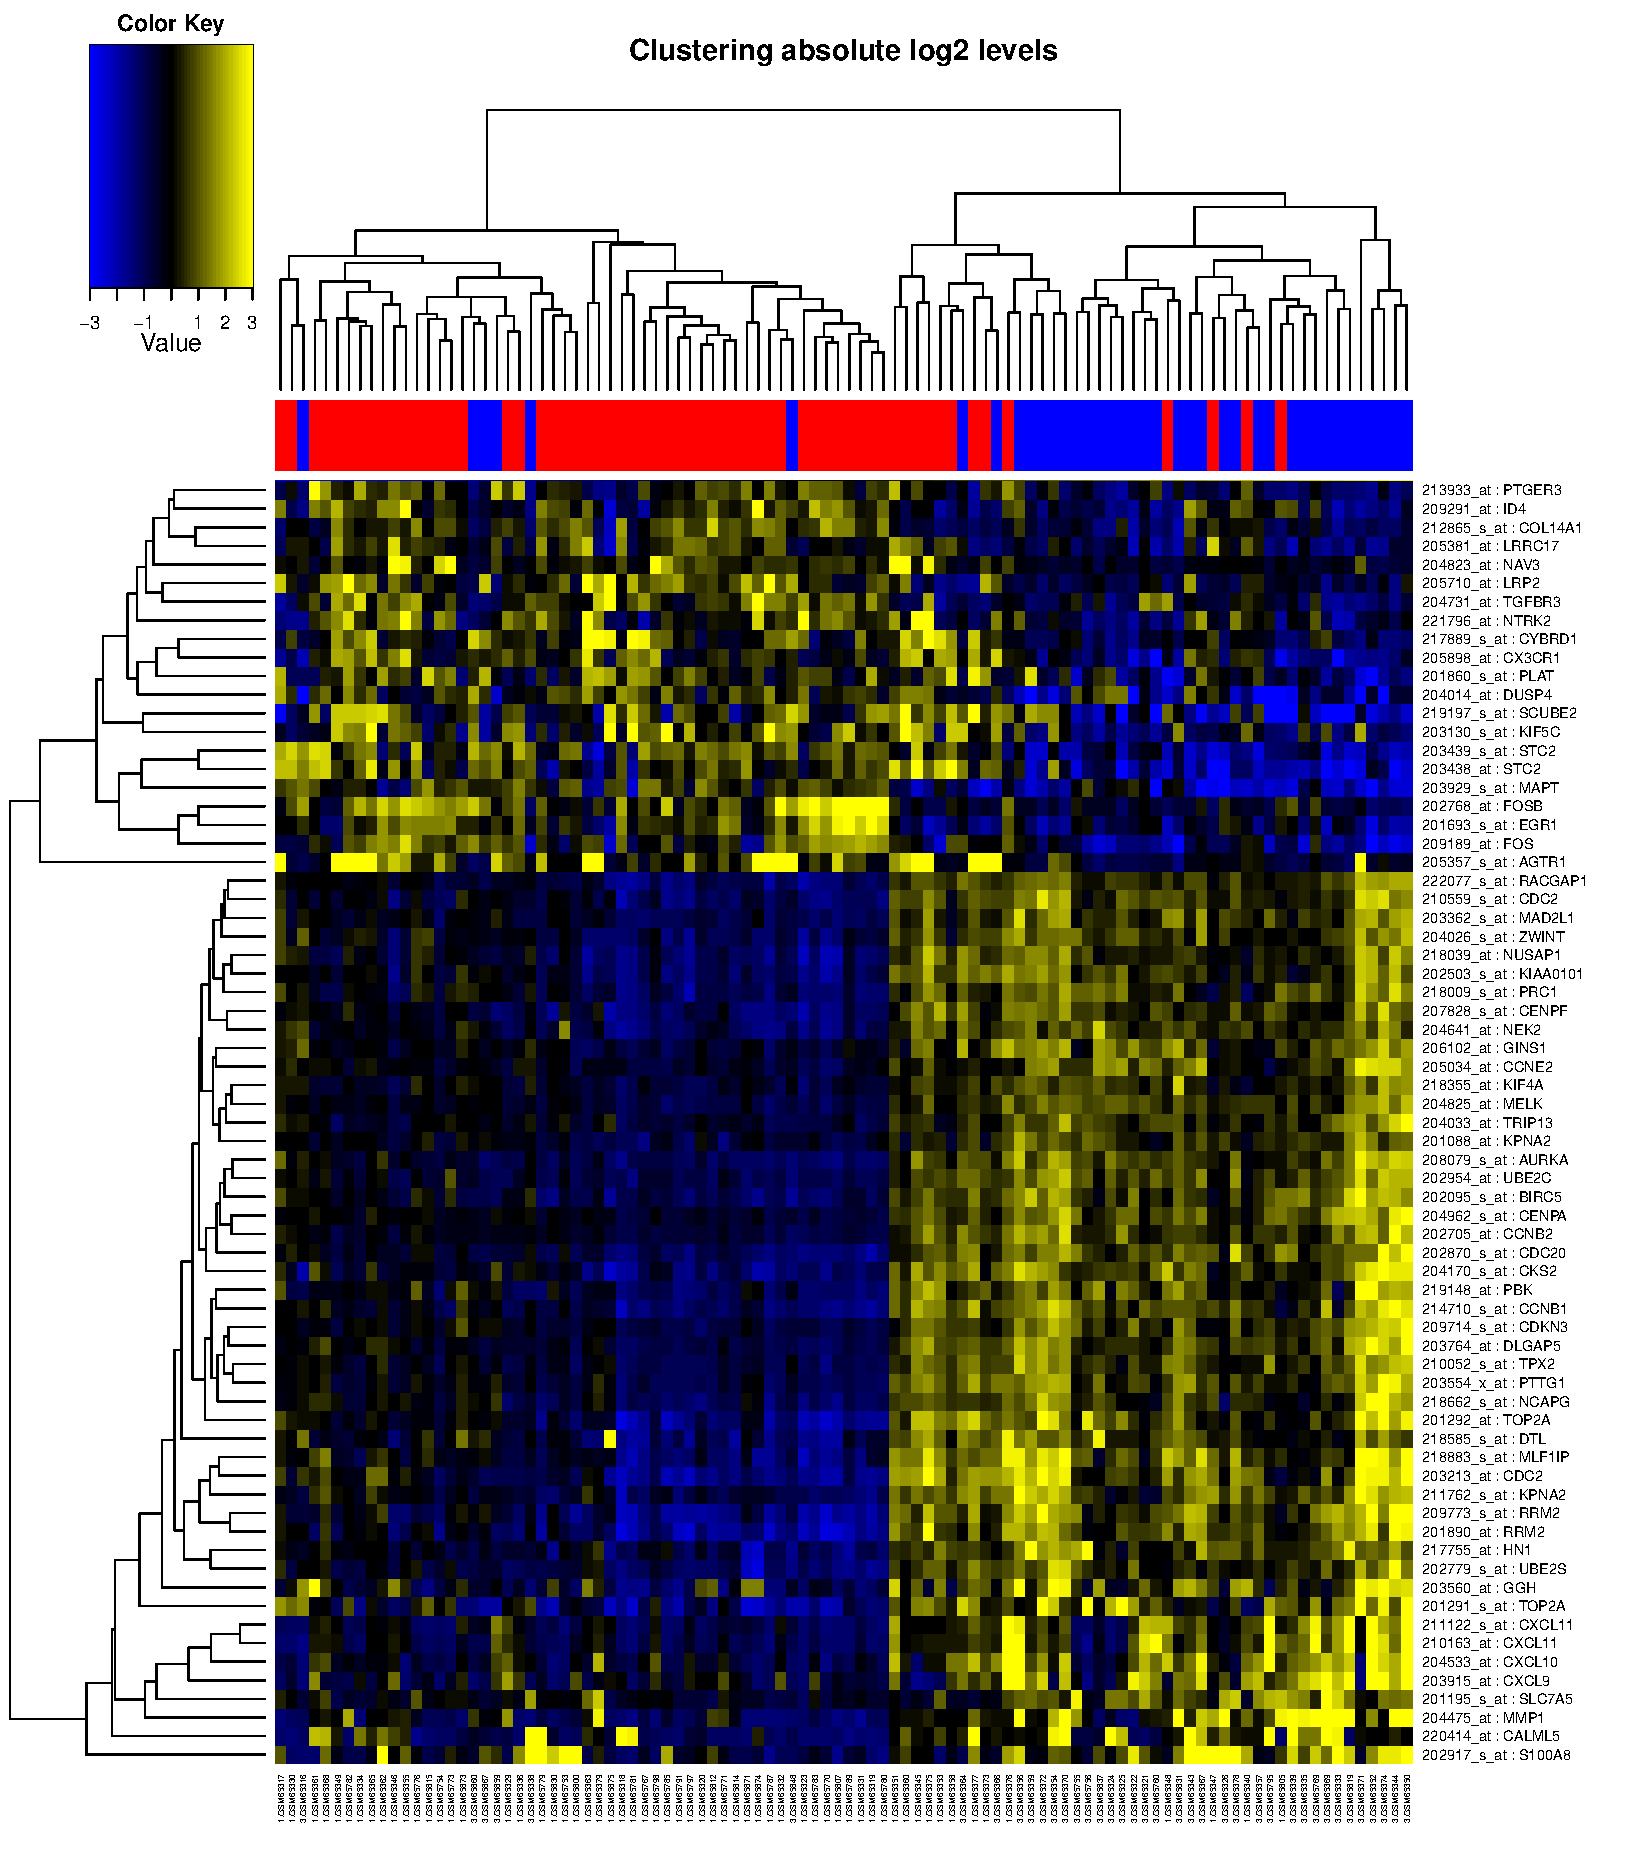
\includegraphics[scale=0.43]{docs/grade1and3differentiallyexpressed}
\caption{Grade 1 and Grade 3 Differentially Expressed.}\label{grade13diff}
%\end{figure}
\end{wrapfigure}
Our method of assessing histological grade of primary breast cancer consists of three phases. The first phase is
a semi-supervised ranking of genes and grade 1 and grade 3 tumors based on maximum differential
expression. The second phase consists of selecting a set of genes that are up-regulated with 
grade 3 tumors and down regulated in grade 3. In the third phase, we generated two groups of tumor samples.
Classification of the grade 2 tumors is then performed using these groups as models. Below we expand upon
our process in detail.\\
The gene signature identification process consisted of assessing the Sotiriou breast cancer data set with Genomics Portals (genomicsportals.org).
Genomics portals performs differential analysis on genes and samples using the CLEAN algorithm\cite{CLEAN}. 
CLEAN co-clusters
the genes and sample grades hierarchically, using data from the dataset and a database of known gene functional groups. Highly differentially
expressed genes were identified with a p-value of .001, and fold change over expression level of 2. The results of this analysis
were inspected in genomics portal's Treeview navigator\cite{Treeview}, and the visually most cohesive up-regulated set of genes
corresponding to grade 3 tumors were selected as our gene signature Figure \ref{grade13diff}. 
Inspection with Treeview failed to suggest a 
visually significant cluster of down-regulated genes for grade 3 tumors, therefore only up-regulated ones were included in our model. 
We acquired a set of 49 differentially expressed up-regulated grade 3 tumor genes from this analysis.
As expected most of those genes turned out to be cell proliferation and cell cycle regulators, notably among them were:
\begin{itemize}
\item Chemokines (known to mediate cell migration and proliferation)
\item Cyclins (control the progression of cells through the cell cycle by activating cyclin-dependent kinase-cdk enzymes)
\item Cyclin-dependent kinase inhibitors  (interact with, and dephosphorylate CDK kinase,  thus preventing their activation; reported to be deleted, mutated, or over-expressed in several kinds of cancers)
\item Aurora Kinase A/ Breast Tumor-Amplified Kinase (involved in microtubule formation and stabilization at the spindle pole during chromosome segregation, may play a role  in tumor development and progression).
\item Ubiquitin-conjugating enzyme E2S (required for cell cycle progression by degradation of mitotic cyclins, consequently, may be involved in cancer progression).
\end{itemize}

\begin{wrapfigure}{l}{0.65\textwidth}
$$
Centroid(Grade_X)= \left[              \underset{x\in X}     \sum{  { {x_1}    \over {| X |} } }   ,   
 \underset{x\in X}     \sum{  { {x_2}    \over {| X |} } },
\ldots ,
 \underset{x\in X}     \sum{  { {x_{| gene signature |}}    \over {| X |} } }                 \right] 
$$
\caption{Grade Gene Expression Centroid Generation.}\label{centroid}
\end{wrapfigure}
Using the selected set of 49 genes as a signature we supposed a $|$gene signature$|-$dimensional subspace to build our model.
Withing the subspace, we used the clinically provided grade labels to generate centroids for the two , 1 and 3 - grade, groups following
the expression (Figure \ref{centroid}) . Noise suppression refinement was performed by removing samples that deviated from the group cluster
centers by more than 2 standard deviations of the cluster's mean variance.\\

\begin{wrapfigure}{r}{0.60\textwidth}
%\begin{figure}
\centering
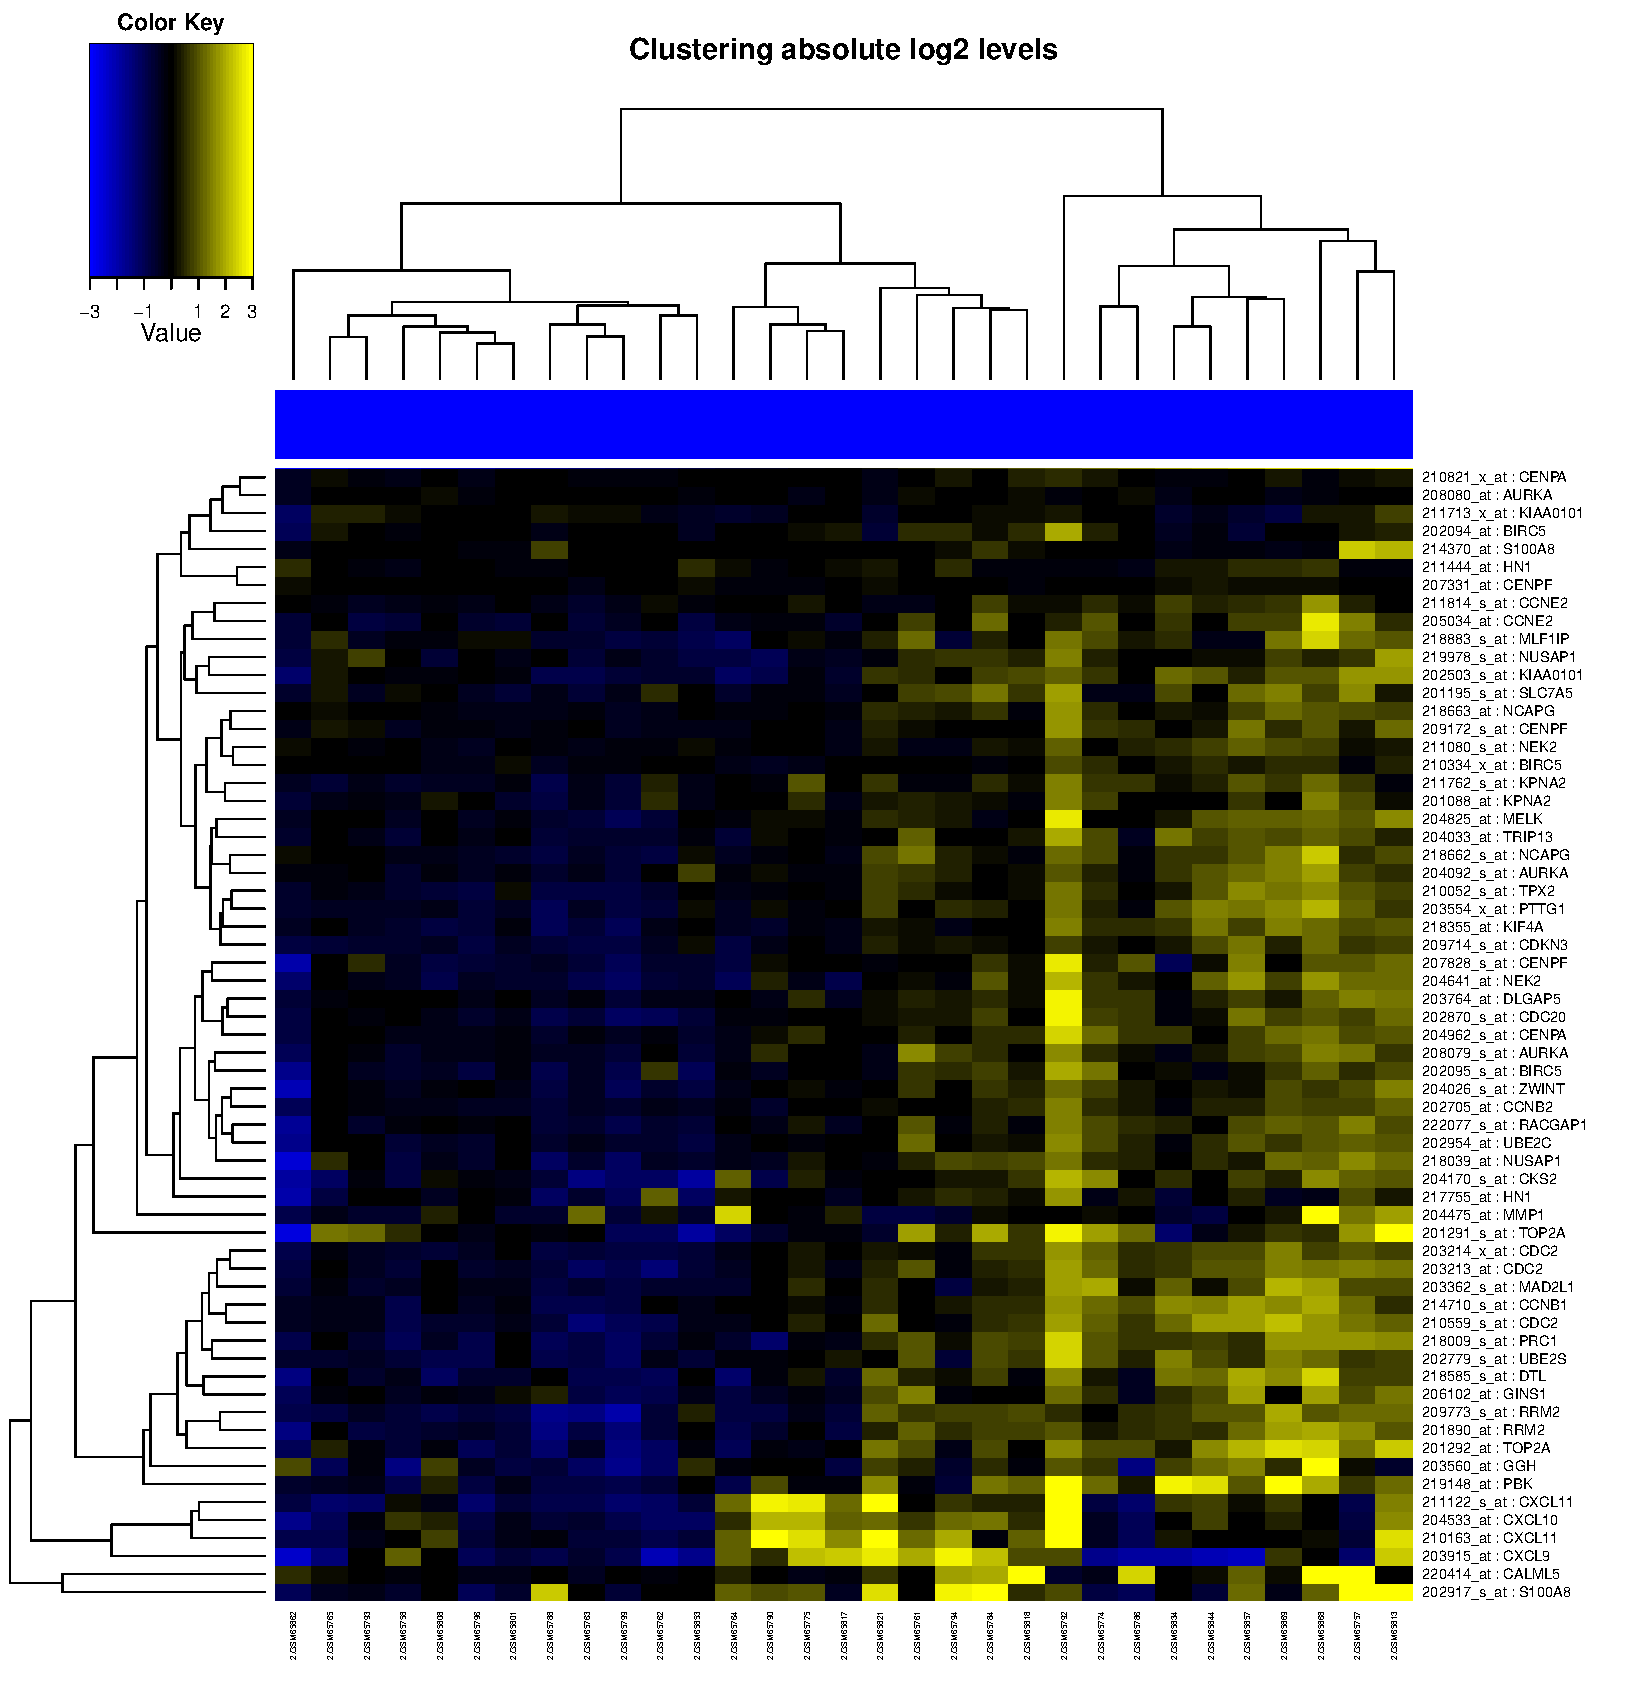
\includegraphics[scale=0.33]{docs/grade2onupregulated3}
\caption{Grade 2 Differentially Expressed Genes from Grade 1 and Grade 3.}\label{grade2up}
%\end{figure}
\end{wrapfigure}
For visual assessment of our analysis, we queried the grade 2 tumors against the grade 1 and 3 differentially expressed genes. The resulting chart
shows a distinct clustering between the grade 1-like and grade 3-like tumors that follow approximately 
the grade 3 and grade 1 distributions. Assuming the dataset comprises the actual distribution 
of grade 1 to grade 3 tumors, approximately 55:64 for grade 1 and grade 3 respectively (Figure \ref{grade2up}) we reassert our hypothesis
of the lack of a grade 2 class distinction.

Classification of grade 2 tumors was then computed by nearest centroid under the euclidean norm following the method in Figure \ref{classify}.
Other distance norms could easily be substituted in place of euclidean, however in this analysis we assumed expression levels were orthogonal
and linear. The new classifications were then used to recompute the KM-Survival analysis on tumor grades 2A (or grade 1-like) and 2b (or grade 3-like).
\begin{wrapfigure}{l}{0.5\textwidth}
 $$
Grade(X) = \underset{C \in Centroids} {\mathrm{argmin}} ~ \left( \sqrt{\sum_{g\in genelist}{ (X_{g} - C_{g})^2}}\right)
$$
\caption{Nearest Centroid Classification.}\label{classify}
\end{wrapfigure}

\subsection{Unsupervised Machine Learning Methods}
In addition to the use of genomics portals to identify differentially expressed genes, two common unsupervised machine learning techniques were
used to classify histological grades based on genetic expression. The first method used was the K-Means method. We will forgo an exhaustive explanation
of K-Means here as it is a long known method with many descriptions and analysis available online. K-Means is an unsupervised clustering method
that attempts to minimize the inter-cluster distance on a set of N points and K cluster assignments. The method is greedy and iterative, with few guarantees
on optimality, however combined with random starts, the overall performance of K-Means is actually quite good for spherical clusters\cite{kmeans}. 
For our testing, following our aforementioned hypothesis of the existence of only two genetically identifiable tumor grades (low and high), we performed
100 tests using K-Means on 50:50 training:test data comprising grade 1 and grade 3 tumors. The reclassification accuracy results are given below.\\
%\begin{wrapfigure}{r}{0.2\textwidth}
\begin{center}
\begin{tabular}{| l | c | }
    \hline
    Mean & 0.8382  \\ \hline
    Mode & 0.84 \\ \hline
    Min & 0.58  \\ \hline
    Max & 0.94  \\ \hline
     Var &  0.00315  \\ \hline
  \end{tabular}
\end{center}
%\end{wrapfigure}

From the results it is clear there is significant error in the upper and lower bounds for accuracy. This though partially due to the K-Means algorithm
itself, may have resulted from a badly conditioned training and test dataset split. As 50\% grade 1 and 50\% grade 3 would suggest the optimal split,
we assert that the actual min accuracy performance is slightly lower than the real performance of K-Means, while the max is no better than could
ideally be achieved from random 50:50 splitting.\\

The second unsupervised method, Projection to Latent Structures Regression (or Partial Least Squares Regression, \emph{PLSR})\cite{Wold1} proved to 
be slightly less accurate in its ability to correctly classify data. Despite its accuracy performance shortcomings, it did however
perform well in its ability to identify highly differentially expressed genes. The explanation of these results is likely due to PLSR's maximization of the covariance
between input data and a set of continuous output training vectors. Though the histological grade is a well ordered set, it is not continuous, and therefor fails to
exploit some of the benefits of a covariance maximization algorithm. The top grade to expression covariance genes (loading vectors of PLSR) are listed below:
\begin{center}
\begin{tabular}{| l | l | l |}
\hline
CALML5 & 51806 & calmodulin-like 5\\ \hline
PBK & 55872 & PDZ binding kinase\\ \hline
RRM2 & 6241 & ribonucleotide reductase M2\\ \hline
NEK2 & 4751 & NIMA (never in mitosis gene a)-related kinase\\ \hline
CCNE2 & 9134 & cyclin E2 \\ \hline
 \end{tabular}
\end{center}

%Computed centroids for grades 1 and 3 based on the 49 up-regulated genes identified with genomic portals.\cite{Treeview},\cite{CLEAN}

%Used those centroids to reclassify grade 2 tumors using Nearest Centroid based on Euclidean distance.

%* Projection to Latent Space Regression (PLSR) on 49, 7231, and 11467 genes.
%on 50:50 train, test data. 
%* Identifies 6 genes: 2 calcium related proteins and 4 chemokines
%* Unsupervised k-means was
%  applied, with similarly poor classification     performance.
%* Performed similar analysis with PAM50 
%* Qualitatively the heatmap results were worse, as PAM50 is for subtype classification.
%* Interestingly, nearest centroid assignment was almost identical.
%Up-regulated genes from grade 3 and 1 differential expression applied to grade 2 tumors (Figure \ref{grade2up})

\section{Results and Discussion}

In order to validate the aforementioned analysis, we created a set of Kaplan-Meier 
(KM) survival curves. These curves show that our gene sets and classification 
methods provide results that are at least as successful as those in the Sotiriou 
paper at separating the grade 2 tumors into two disjoint sets. 
For context, figure \ref{1S} shows three KM curves from the Sotiriou paper:
\begin{figure}
%\begin{figure}
\centering
\includegraphics[scale=0.35]{docs/Figure1S}
\caption{Kaplan-Meier curves from Sotiriou, et al.}\label{1S}
%\end{figure}
\end{figure}
Graph \ref{1S} shows the original data from their analysis. Grade 1, 2, and 3 tumor 
curves clearly separate from each other, clearly creating 3 separate and distinct 
classes. However, we would like to demonstrate that grade 2 tumors should 
actually be classified as either grade 1 or grade 3. \\

This is analysis is begun in graph B, as Sotiriou et al. used something 
they called the “Gene Expression Grade Index” (GGI) to reclassify 
grade 2 tumors. This index is shown below:
$$
GGI = scale\left( \sum_{j\in G_3}{ x_j } - \sum_{j\in G_1}{ x_j } - offset  \right)
$$
Gene Expression Grade Index, a tumor reclassification formula
If the value of this formula was negative for a grade 2 sample, 
the sample would be reclassified as a grade 1 tumor, while a positive 
value would indicate a grade 3 tumor. Graph C shows all samples reclassified using the GGI.
In our analysis, we chose a different re-classification technique. 
This was described above as the nearest-centroid method. We reclassified 
each grade 2 sample to either grade 1 or 3 to produce the graph in Figure \ref{3S}.\\



Using Figure \ref{3S} we were able to see a difference between our re-graded curve 
and the original. Our reclassification actually intensified the gap between the grade 1 and 3 curves.
Figure \ref{4S} shows the integration of grade 2 reclassifications in Figure  \ref{3S} with 
the original grade 1 and 3 samples. That is, the curve labeled “grade 1” in 
Figure  \ref{4S} includes all of the original grade 1 samples and grade 2 samples 
that were classified as “1-like”, while the grade 3 curve contains the original
 grade 3 samples and the grade 2 samples that were classified as “3-like”. 
The graph is analogous to the Sotiriou analysis shown in Figure \ref{4S}-C.
\begin{figure}
%\begin{figure}
\centering
\includegraphics[scale=.55]{docs/Figure3S}
\caption{Reclassification of grade 2 samples using nearest-centroid method.}\label{3S}
%\end{figure}
\end{figure}

%\begin{wrapfigure}{r}{.6\textwidth}
\begin{figure}[t]
\centering
\includegraphics[scale=0.60]{docs/Figure4S}
\caption{All samples reclassified using the nearest-centroid method.}\label{4S}
\end{figure}
%\end{wrapfigure}
 \begin{wrapfigure}{c}{0.65\textwidth}
%\begin{figure}
\centering
\includegraphics[scale=0.4]{docs/Figure5S}
\caption{All samples reclassified using PAM50 genes.}\label{5S}
\vspace{-50pt}
%\end{figure}
\end{wrapfigure}
For a control, we thought it might be interesting to run a similar 
analysis using the PAM50 geneset, a list of genes known to be differentially
 expressed across breast cancer tumor subtypes. The reclassification using 
the PAM50 genes (and nearest-centroid) is shown in the KM curve in Figure \ref{5S}.


\subsection{Results}
 \begin{wrapfigure}{h}{0.60\textwidth}
%\begin{figure}
\centering
\vspace{-30pt}
\includegraphics[scale=0.45]{docs/Figure5S}
\caption{ KM curve of relapse free survival over time in ER positive versus ER negative samples.}\label{1B}
\vspace{-10pt}
%\end{figure}
\end{wrapfigure}
Baseline KM curves Based on the study’s data without any reclassification, KM survival analyses with outcome 
defined as relapse free survival were performed for samples in the KJ125 set.   KM analysis 
was performed for ER positive samples versus ER negative samples in the cohort (Figure \ref{1B}). 
The ER negative samples tended to have worse prognosis than ER positive samples although 
the difference did not reach statistical significance. This trend is consistent with literature 
evidence that ER negative tumors are more malignant.  \\

A KM curve was next generated for histologic grade among samples in the KJ125 cohort.  
Histologic grades 2 and 3 were associated with worse prognosis with regard to relapse 
free survival than grade 1 (Figure \ref{2B}).  Interestingly, there was no observed difference 
between grade 2 and 3 tumors.  \\

Unsupervised clustering between grade 1 and grade 3 tumors within only the 
KJX64 set was performed, which identified a list of 30 probe sets comprising 
29 genes that are differentially expressed between grade 1 and grade 3 tumors 
(Table \ref{T1}).  Specifically, these genes were upregulated in histologic grade 3 tumors 
and downregulated in histologic grade 1 tumors.  \\



\begin{table}
\begin{tabular}{| l | l | l | l | }
    \hline
202095\_s\_at & BIRC5 & 332 & baculoviral IAP repeat-containing 5\\ \hline 
214710\_s\_at & CCNB1 & 891 & cyclin B1\\ \hline 
210559\_s\_at & CDC2 & 983 & cell division cycle 2, G1 to S and G2 to M\\ \hline 
202870\_s\_at & CDC20 & 991 & cell division cycle 20 homolog (S. cerevisiae)\\ \hline 
209714\_s\_at & CDKN3 & 1033 & cyclin-dependent kinase inhibitor 3\\ \hline 
204962\_s\_at & CENPA & 1058 & centromere protein A\\ \hline 
204170\_s\_at & CKS2 & 1164 & CDC28 protein kinase regulatory subunit 2\\ \hline 
203744\_at & HMGB3 & 3149 & high-mobility group box 3\\ \hline 
211762\_s\_at & KPNA2 & 3838 & karyopherin alpha 2 (RAG cohort 1, importin alpha 1)\\ \hline 
203915\_at & CXCL9 & 4283 & chemokine (C-X-C motif) ligand 9\\ \hline 
201890\_at & RRM2 & 6241 & ribonucleotide reductase M2\\ \hline 
209773\_s\_at & RRM2 & 6241 & ribonucleotide reductase M2\\ \hline 
208079\_s\_at & AURKA & 6790 & aurora kinase A\\ \hline 
201291\_s\_at & TOP2A & 7153 & topoisomerase (DNA) II alpha 170kDa\\ \hline 
201195\_s\_at & SLC7A5 & 8140 & solute carrier family 7 (cationic amino acid transporter, y+ system), 5\\ \hline 
218009\_s\_at & PRC1 & 9055 & protein regulator of cytokinesis 1\\ \hline 
202705\_at & CCNB2 & 9133 & cyclin B2\\ \hline 
205034\_at & CNE2 & 9134 & cyclin E2\\ \hline 
203554\_x\_at & PTTG1 & 9232 & pituitary tumor-transforming 1\\ \hline 
204033\_at & TRIP13 & 9319 & thyroid hormone receptor interactor 13\\ \hline 
204825\_at & MELK & 9833 & maternal embryonic leucine zipper kinase\\ \hline 
206102\_at & GINS1 & 9837 & GINS complex subunit 1 (Psf1 homolog)\\ \hline 
202954\_at & UBE2C & 11065 & ubiquitin-conjugating enzyme E2C\\ \hline 
204026\_s\_at & ZWINT & 1130 & ZW10 interactor\\ \hline 
210052\_s\_at & TPX2 & 22974 & TPX2, microtubule-associated, homolog (Xenopus laevis)\\ \hline 
204086\_at & PRAME & 23532 & preferentially expressed antigen in melanoma\\ \hline 
202779\_s\_at & UBE2S & 27338 & ubiquitin-conjugating enzyme E2S\\ \hline 
222077\_s\_at & RACGAP1 & 29127 & Rac GTPase activating protein 1\\ \hline 
218039\_at & NUSAP1 & 51203 & nucleolar and spindle associated protein 1\\ \hline 
218883\_s\_at & MLF1IP & 79682 & MLF1 interacting protein\\ \hline
\end{tabular}
\caption{List of 30 probe sets comprising 29 genes which are upregulated in KJX64 histologic 
grade 3 samples and downregulated in grade 1 samples.}\label{T1}
\end{table}


The centroid-based approach utilizing calculated Euclidean distances was applied to the 
KJ125 samples.   Figure \ref{3B} depicts a KM analysis for relapse free survival based on 
centroid-based reclassification of all KJ125 samples. This includes histologic grades 1, 2, 3, 
and those with histologic grade not available.  Grade 1-like tumor samples were associated 
with significantly lower risk of disease relapse.  Figure \ref{4B} depicts the KM analysis for 
centroid-based reclassification of only grade 2 tumor samples in the KJ125 set and 
also demonstrates better prognosis for those samples reclassified as grade 1-like. 
\begin{wrapfigure}{r}{0.5\textwidth}
%\begin{figure}
\vspace{10pt}
\centering
\includegraphics[scale=0.45]{docs/Figure2B}
\caption{ KM curve of relapse free survival over time in groups based on histologic grades.}\label{2B}
%\end{figure}
\end{wrapfigure}


 %\begin{wrapfigure}{r}{.6\textwidth}
\begin{figure}[b!]
\centering
\includegraphics[scale=0.5]{docs/Figure3B}
\caption{ KM analysis of relapse free survival among all 
KJ125 tumors reclassified as 1-like or 3-like based on 
microarray gene expression profiles.}\label{3B}
\end{figure}
%\end{wrapfigure}
Next, the list of the 29 differentially expressed genes in the above table was queried against 
the RNAseq gene expression data from by PAM50 subtype in TCGA \cite{Nature1}.  
The clustering is demonstrated in Figure \ref{5B}.  There is a cluster of 108 samples with 
increased expression of the genes of interest, which can be considered grade 3-like. 
 Interestingly, nearly half of the samples in this cluster were basal-like tumors based on 
PAM 50 signature (Table \ref{T2}).  In addition, 64\% of all basal-like tumors in the 
analysis were found in this cluster. Furthermore, there were only 3 luminal A subtype
 tumors within the grade 3-like cluster which comprised only 1.4\% of luminal A tumors
 in this dataset. These findings are consistent with observations that luminal A subtype
 tumors are less aggressive than basal-like tumors and serves as a validation of our 
generated gene list. The TCGA paper does not provide survival data, which would 
be another interesting validation to be explored in the future.\\
% \begin{wrapfigure}{r}{0.64\textwidth}
\begin{figure}
\centering
\includegraphics[scale=0.60]{docs/Figure4B}
\caption{ KM analysis of relapse free survival between 
histologic grade 2 tumors in KJ125 set reclassified as 
1-like or 3-like based on gene expression profiles.}\label{4B}
\end{figure}
%\end{wrapfigure}

 \begin{wrapfigure}{r}{1.\textwidth}
%\begin{figure}
\centering
\includegraphics[scale=0.80]{docs/Figure5B}
\caption{ Query of TCGA RNAseq gene expression data with our generated list of genes 
based on Sotiriou microarray expression profiles.  There is a cluster of increased gene 
expression (yellow box) containing 108 samples which can be considered grade 3-like.}\label{5B}
%\end{figure}
\end{wrapfigure}


 \begin{wrapfigure}{r}{0.64\textwidth}
\begin{tabular}{| l | l | l | l | }
    \hline
\textbf{Subtype} & \textbf{Number of} & \textbf{Number of tumors in } & \textbf{Percent}\\  
 &   \textbf{tumors}  & \textbf{cluster of increased} & \\
 &  \textbf{ (N=434)} & \textbf{expression (N=108)} & \\
\hline
Normal & 6 & 2 & 33\% \\ \hline 
 LumA & 201 & 3 & 1.4\% \\ \hline 
 LumB & 101 & 35 & 34.6\% \\ \hline 
 Her2 & 47 & 17 & 36.2\% \\ \hline 
 Basal-like & 79 & 51 & 64.6\% \\ \hline 
\end{tabular}
\caption{Query of TCGA RNAseq gene expression data with our generated list of genes,
 clustered by PAM50 subtype.  The cluster of increased expression (grade 3-like) has a preponderance 
of Basal-like tumors and paucity of luminal A tumors.}\label{T2}
\end{wrapfigure}

We further explored the gene list of any functional annotation utilizing resource tools 
\emph{DAVID} and \emph{KEGG}\cite{Huang1}\cite{Kanehisa1}\cite{Kanehisa2}\cite{Ogata1}.  These analyses found that our gene list 
was functionally enriched for 3 pathways: cell cycle regulation, progesterone-mediated 
oocyte meiosis, and ubiquitin-mediated protein degradation in figures \ref{6B}, \ref{7B}, and \ref{8B}. 
 These pathways are consistent with the known features of advanced histologic 
grade such as mitosis and dedifferentiation.  The majority of genes in our list
 overlapped with the list generated by Sotiriou et al. Several of the selected 
overlapping genes are shown in Table \ref{T3}.  Notably, these genes are known to 
be associated with oncologic processes in multiple other organs according to 
queries of the GeneCards web tool (www.genecards.org).  


 %\begin{wrapfigure}{r}{.7\textwidth}
\begin{figure}
\centering
\includegraphics[scale=0.65]{docs/Figure6B}
\caption{List of differentially upregulated genes in histologic 
grade 3 tumors is enriched for the pathway of cell cycle regulation.}\label{6B}
\end{figure}
%\end{wrapfigure}


 \begin{wrapfigure}{r}{1.\textwidth}
%\begin{figure}
\centering
\includegraphics[scale=0.50]{docs/Figure7B}
\caption{ List of differentially upregulated genes in 
histologic grade 3 tumors is enriched for the pathway 
of progesterone-mediated oocyte maturation.}\label{7B}
%\end{figure}
\end{wrapfigure}

 \begin{wrapfigure}{r}{0.64\textwidth}
%\begin{figure}
\centering
\includegraphics[scale=0.45]{docs/Figure8B}
\caption{ List of differentially upregulated genes in histologic grade 
3 tumors is enriched for the pathway of ubiquitin-mediated protein 
degradation.}\label{8B}
%\end{figure}
\end{wrapfigure}

\begin{table}
\begin{tabular}{| l | l | l | l | }
    \hline
\textbf{Gene} & \textbf{Protein} & \textbf{Function} & \textbf{Associated diseases}\\ \hline 
TPX2 & TPX2, microtubule & Required for assembly of mitotic & Hepatocellular \\
 &  -associated, homolog  & spindles & carcinoma \\
 & (Xenopus laevis) &   &  Colorectal cancer
\\ \hline
CCNB1 & Cyclin B1 & Initiates mitosis & Many cancers\\ \hline 
CDC20 & cell division cycle 20 & Cell cycle regulation & Ataxia-telangiectasia \\
 & homolog (S. cerevisiae)  & &  ($\uparrow$ cancer risk) 
\\ \hline
PTTG1 & pituitary tumor- & Chromosome stability, negatively & Thymic hyperplasia\\
 & transforming 1 & regulates TP53 &  Nelson syndrome \\
 & & & (pituitary adenoma)
\\ \hline 
UBE2C & ubiquitin-conjugating & Targeting proteins for degradation & Esophageal carcinoma \\
 & enzyme E2C  & & Papillary thyroid \\
 & & & carcinoma
\\ \hline 
KPNA2 & karyopherin alpha 2 & Nuclear protein import & Nijmegen breakage \\
 & (RAG cohort 1, importin & & syndrome ($\uparrow$ cancer \\
 & alpha 1) &  &   risk) 
\\ \hline 
BIRC5 & baculoviral IAP repeat- &  Inhibits apoptosis and promotes & Cervical cancer \\
 & containing 5 & cell proliferation &  Laryngeal carcinoma
\\ \hline
\end{tabular}
\caption{Selected genes of interest which were identified to be upregulated in 
Grade 3 tumors in our analyses as well as the analyses by Sotiriou.  
These genes are recognized to be associated with other oncologic 
processes and systemic disorders associated with cancer risk.}\label{T3}
\end{table}


\subsection{Discussion}
As shown above, our discovered geneset and reclassification method were 
able to split grade 2 tumors into two disjoint sets. These sets may be more 
helpful in tumor diagnosis and treatment, as grade 2 diagnoses are currently
 not considered “not informative for clinical decision making” \cite{Sotiriou1}.
Our methods were able to produce a result that was slightly better than the 
Sotirou paper at a significant p-value (p=0.05). In addition, using the PAM50
 geneset, we were able to reproduce these results and achieve an almost 
identical graph. This was unexpected, as PAM50 genes are known to 
separate samples based on their subtype rather than their grade. However, 
it is notable to mention that grade 1 and 3 tumors are more likely to be Basal 
and Luminal tumors, respectively. This explains the similarity between our 
and the PAM50 results.\\

Limitations to the study include pathologist variation and possible misclassification, region or 
race specific differences since two populations are presented, and complications to analysis with ER status. \\

In our study, we only used estrogen receptor positive tumors to look at the differentially 
expressed genes. Thus the conclusions are limited to only the ER positive tumors and 
inferences cannot be made as to ER negative tumors. Future work would include looking into the
 differentially expressed genes in both estrogen receptors positive and negative tumors and then
 compare the gene list between each other. This can shed light on which specific genes are dependent 
on the ER status of tumors. \\

In addition, looking at expression signatures based on AJCC staging classification systems 
may decease some data set variation. The main criteria of the AJCC staging 
systems include tumor size, lymph node status, and distant metastasis. Future studies should 
also examine age of onset, races and geographic regions to look for variability and to improve 
treatment for different groups.\\ 

\subsubsection{Caveats}
While we were able to analyze the given dataset in an unbiased manner, 
there was no way for us to control the data given to us. In that vein, we 
were unable to control the research population for tumor size, age, 
margin, ER status, or lymph node status.\\

On a similar note, there was no way for us to alter our survival analysis 
based on what treatments were being offered to each patient. The 
possibility that different patients were participating in different treatments 
throughout their lives is enough to alter the confidence intervals on our KM 
curves.

\subsubsection{Future Work}
Our work with the Sotirou paper was only able to reproduce their analysis 
and improve upon it slightly. There is still a large amount of work that could 
be done to further validate our methods, as well as to delve deeper in to the 
work done by both our teams.\\

Firstly, in order to prove our work we would like to perform validation in
 some other independent datasets. In addition, we could perform a 
prospective study at some point in the future. Unfortunately, this does seem 
unlikely.\\

Moreover, an easier way to validate our results would be to perform the same 
analysis using the Distant Metastasis Free Survival Rate (DMFS). Our work 
solely included Relapse Free Survival (DFS) data.

\bibliography{refs}
\bibliographystyle{ieeetr} \markright{ }
\end{document}
